We conduct our study in a large scale open source software system to distinguish Defect Debt and Bugs. First, we analyze the history of issues in the system, and then we suggest a definition to Defect Debt and to Bugs. Based on this definition we quantify  both on them per release. Second, we analyze the evolution of Defect Debt to understand its impact on future feature addition. Third, based on our metrics we propose a model to Defect Debt.

\vspace{3mm}
\noindent\rqi
\vspace{3mm}

\noindent\textbf{Motivation:} Intuitively we know that different defects has different impacts in software quality. We hypothesize that defects in a project can be categorized in two different classifications. First, bugs which are high priority defects usually fixed near to its reported date. Second, Defect Debt which are defects that lingers in the system until an opportunity to fix it appears. Answering this research question, will provide us a way to identify and quantify Defect Debt .

\vspace{1mm}
\noindent\textbf{Approach:} To identify defect debt in a software project we first mine its issuer tracker to extract all bug reports available. Then, we link the bug report to the software releases using its reported date. Then we link the commits with bugs trough the commit message.  We analyze then the data for three different patterns, Bugs that were opened and closed in the release. Bugs that were opened in one release and fixed in a future release. Finally, bugs that were opened and was closed with a WONT\_FIX decision or that were opened and after some releases they were not addressed. (The number of releases should vary accordingly with the number of releases of the project analyzed). With the analysis done, we can quantify the results obtained for each category described.

\vspace{1mm}
\noindent\textbf{Result:} Most defects are fixed during the release that they were reported or in the next one. A number of defects reported in the current release will remain in the system for a long time, but eventually get fixed.


\begin{figure}[thb!]
    \caption{Release density evolution}
    \label{fig:release_density}
    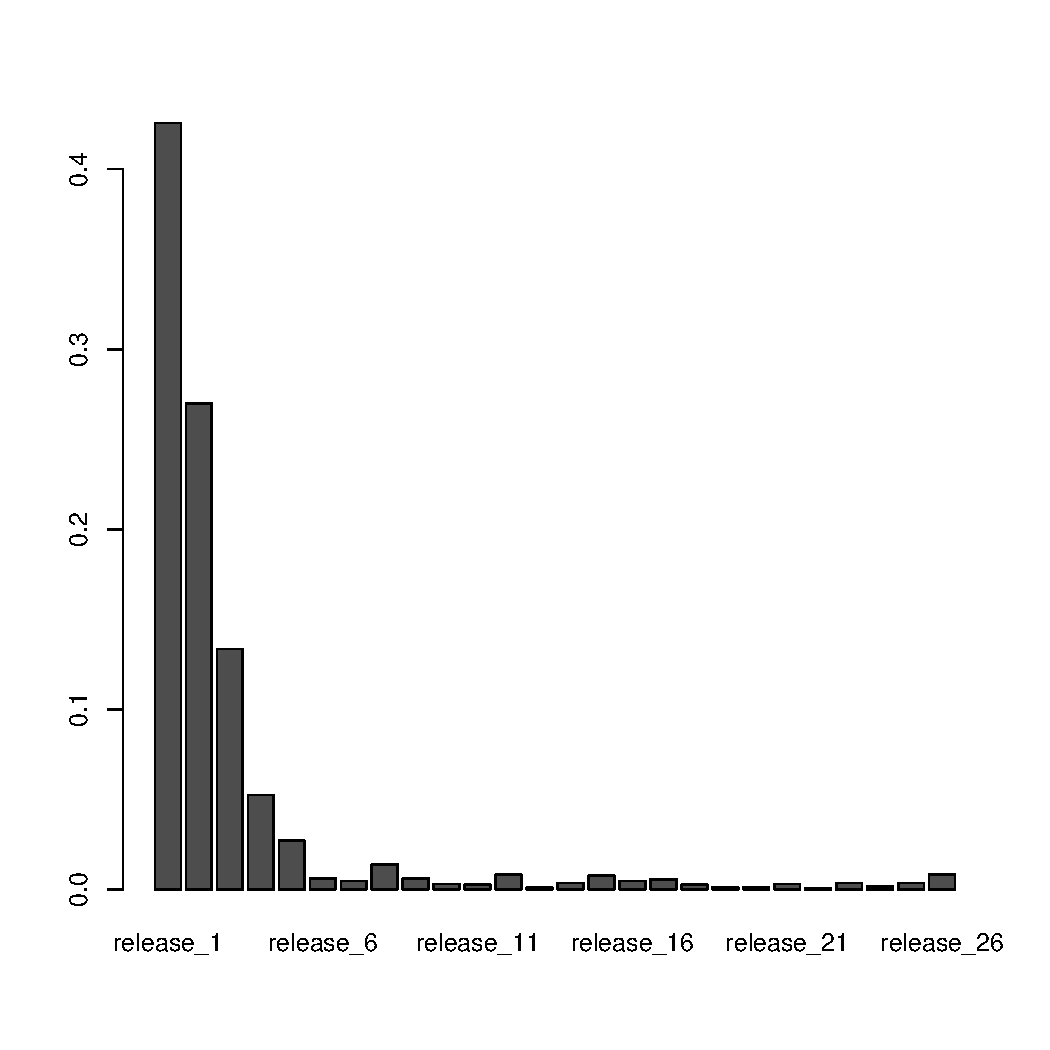
\includegraphics[width=90mm,scale=0.5]{figures/r1}
\end{figure}

\begin{figure}[thb!]
    \caption{Release density evolution}
    \label{fig:release_density}
    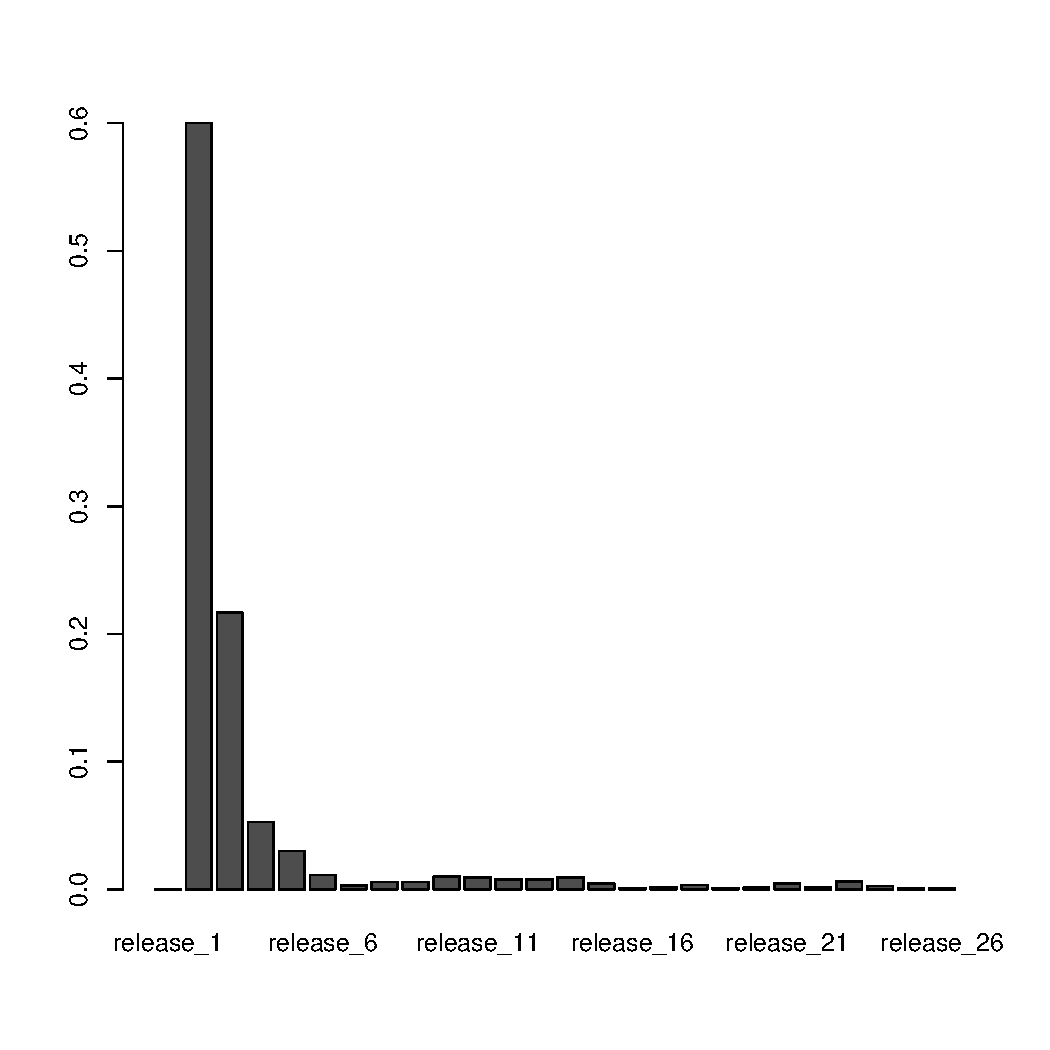
\includegraphics[width=90mm,scale=0.5]{figures/r2}
\end{figure}

\vspace{3mm}
\noindent\rqii
\vspace{3mm}

\noindent\textbf{Motivation:} Technical debt can bring you short term advantage in trade off maintenance costs in the  long run. which means that when well managed technical debt can be used as a tool to achieve projects goals. That been said, we want to know how much is too much when dealing with technical debt. We argue that the amount of technical debt starts to slow down your development is the point to pay off. 

\vspace{1mm}
\noindent\textbf{Approach:} Now that we have an approach to identify defect debt we want to see how it relates with the amount of changes in the project. First we quantify the number of defect debt in the software, then we mine the source code repository to examine the changes. We will find all the changes(commits) related to a specific release using the commit date. Analyzing the commit messages we will categorize the changes of the release to see with the change is due to a bug fix or adding new features. After this analyze we will have the number of commits that were bug fix and the number of commits that were new features. To measure if  a high number of defect debt is preventing new features to be implemented in the project, we analyze if the number of new features are reducing at the same time that the number bug fixes are increasing. We also should expect that a higher number of defects is reported when the number of technical debt is higher in the project.

\vspace{1mm}
\noindent\textbf{Result:} The number of open defects increases during the project life-cycle. Defect Debt has growth peaks, but eventually get removed in future releases. Analyzing the feature addition and the defect debt graph we found that the introduction of defect debt does not impact the number of  feature addition per release. 

\begin{figure}[thb!]
    \caption{Release density evolution}
    \label{fig:release_density}
    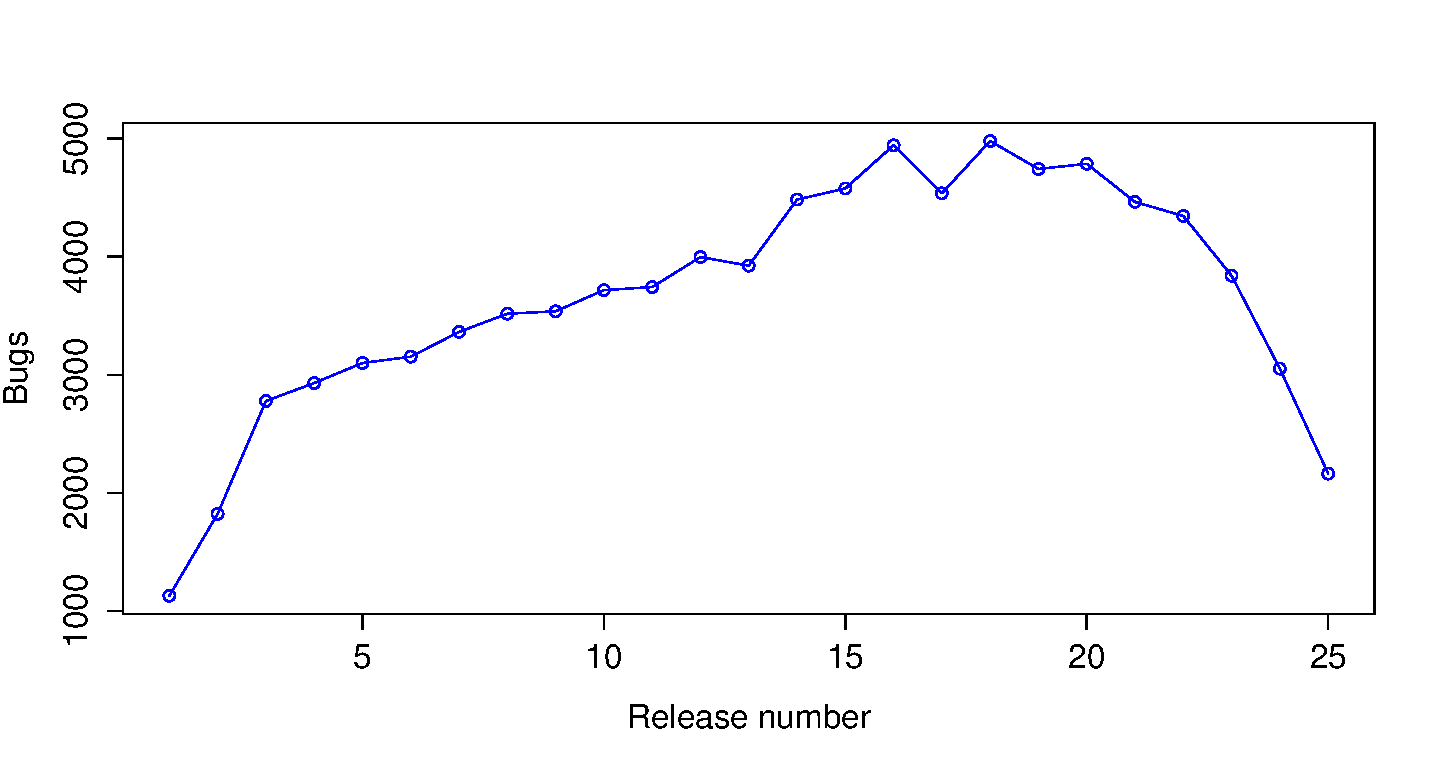
\includegraphics[width=90mm,scale=0.5]{figures/number_of_bugs_releases}
\end{figure}

\begin{figure}[thb!]
    \caption{Release density evolution}
    \label{fig:release_density}
    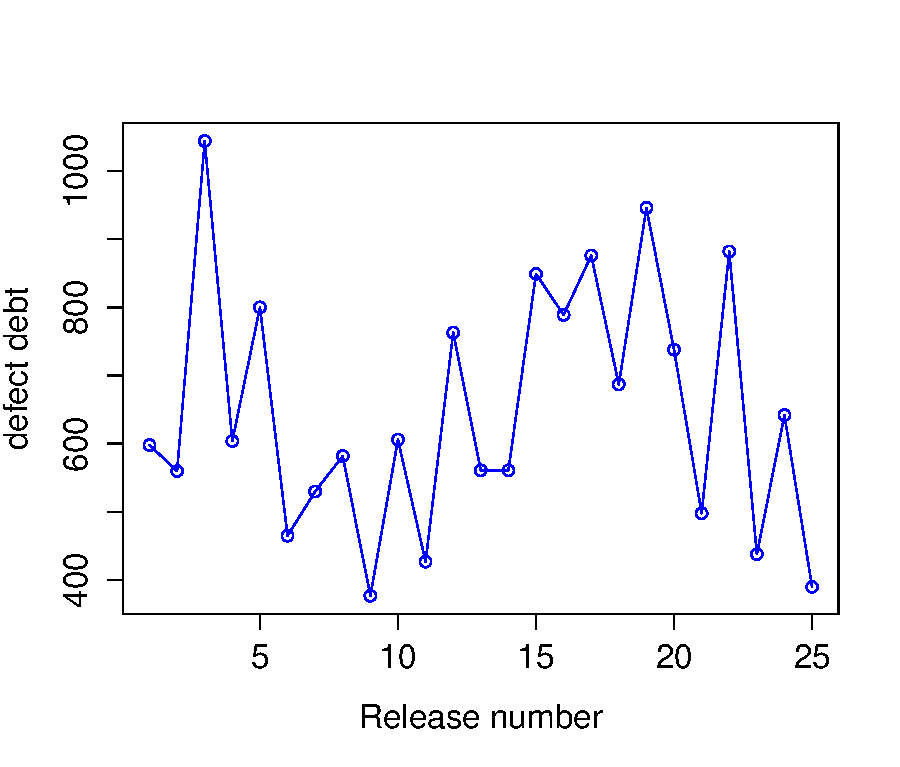
\includegraphics[width=90mm,scale=0.5]{figures/technical_debt}
\end{figure}

\begin{figure}[thb!]
    \caption{Release density evolution}
    \label{fig:release_density}
    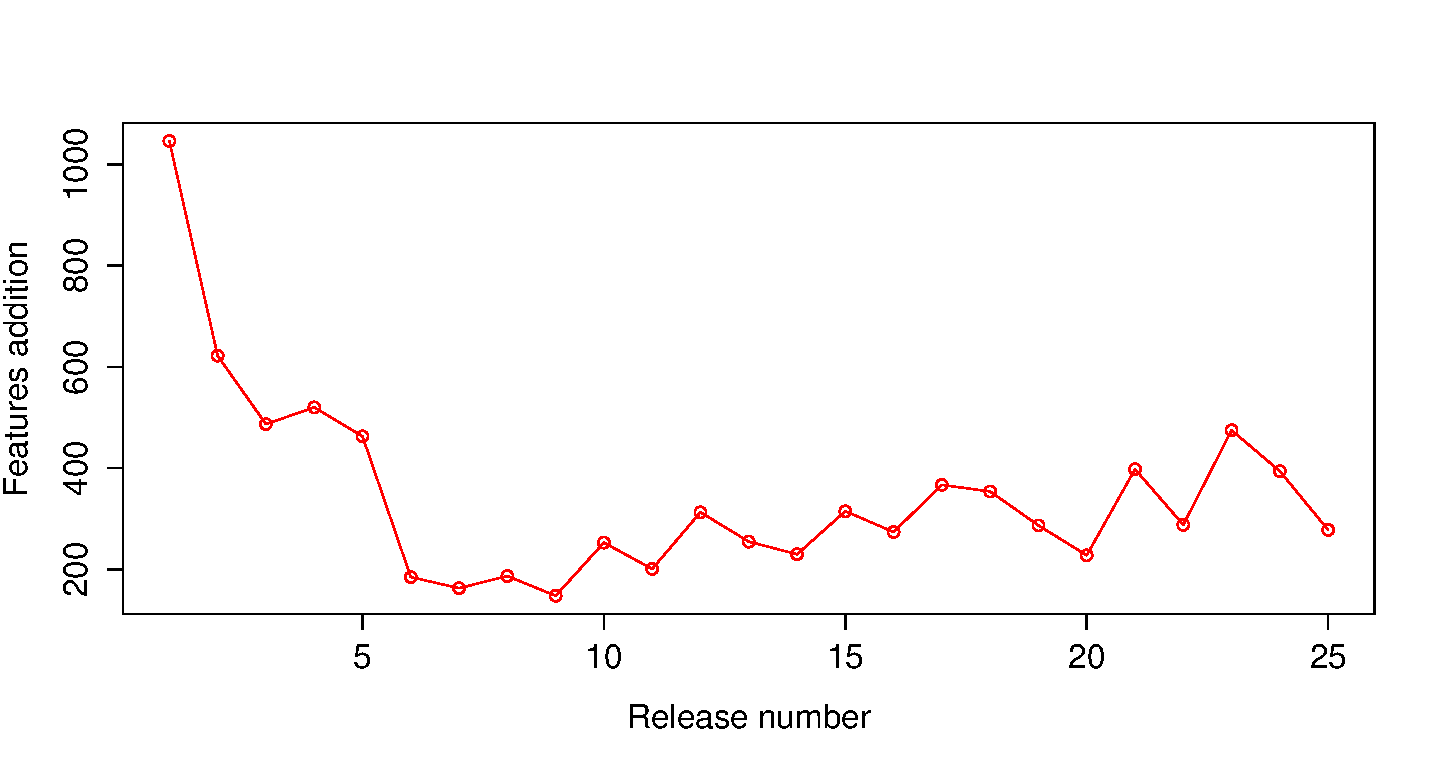
\includegraphics[width=90mm,scale=0.5]{figures/feature_addition_releases}
\end{figure}

\vspace{3mm}
\noindent\rqiii
\vspace{3mm}

\noindent\textbf{Motivation:} Learning from mistakes of the past can be useful in software engineering as well. We want to know if it is possible to determine if a defect are likely to become defect technical debt by analyzing the cases that were identified in RQ1. Answering this question will provide us with more means to effectively manage defect debt by knowing before hand that the specific defect will have to be handled in the future to avoid quality impacts. 

\vspace{1mm}
\noindent\textbf{Approach:} Based on the defect debt identified in the project we will analyze the bug reports looking for patterns in the attributes to build a prediction model. This information will serve as our training set. Then we will run the analyze again using the data from other project to measure the precision of our model. 

\vspace{1mm}
\noindent\textbf{Result:}